\chapter{Conclusions}

\section{Gateway Locations}\label{sec:gateway-locations-conclusions}

% Evaluate the chosen gateway locations and give example of the ranges, etc.
% Also add graphs of recorded gateway ranges from TTN Mapper?
This section will evaluate the chosen gateway locations as described in \cref{sec:gateway-locations} and give some examples of the ranges that can be achieved with them.
The maps used to show range data were taken from the \emph{Advanced Maps} feature of \ac{TTNM}.
Thus, as explained in \cref{subsec:cleaning-collected-data}, they may contain some inaccuracies and outliers.

\subsection{\acf{GHB} student dormitory}\label{subsec:ghb-student-dormitory-range-results}

The MikroTik gateway deployed on top of the \ac{GHB} student dormitory is the gateway with the highest range in Furtwangen among those deployed during this thesis.
This doesn't come as a surprise, given its exposed location on top of a hill plus the height of the building itself.

\begin{figure}[htbp]
    \centering
    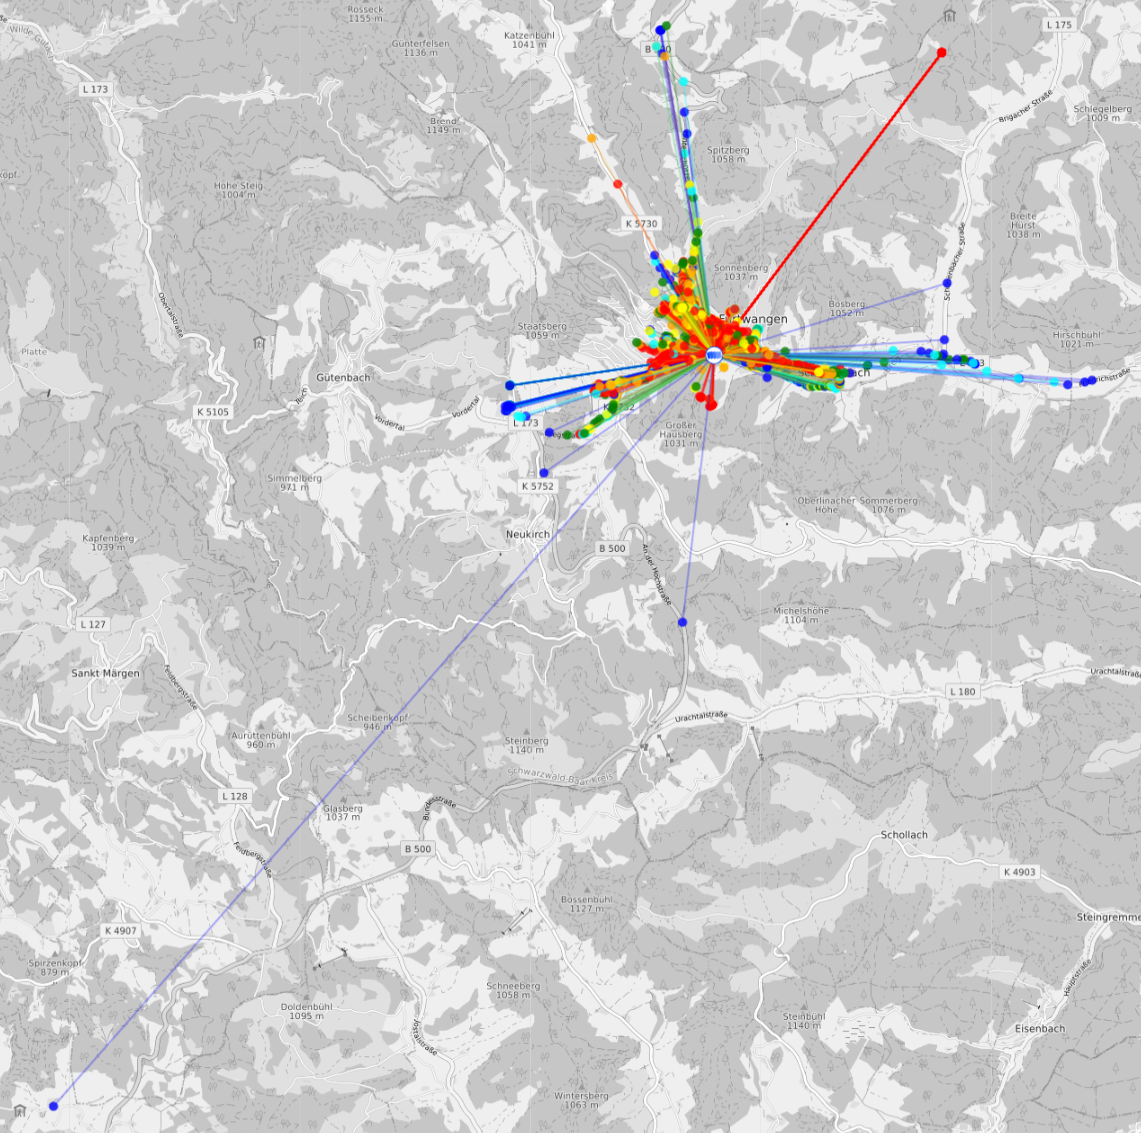
\includegraphics[width=1\textwidth]{pictures/ttn-mapper/gateway-ranges/ghb_mikrotik_gw_range.png}
    \caption{
        Map of some \ac{TTNM} data points taken from the \ac{LoRaWAN} gateway deployed on top of the \ac{GHB} student dormitory.
        The data point on the lower left is the maximum range recorded for this gateway --- \SI{14.2}{\kilo\meter}.
        However, it can be considered an outlier, as the next highest range is \SI{5.3}{\kilo\meter} away from the gateway (on the far right).
    }\label{pic:ghb_mikrotik_gw_range}
\end{figure}

The maximum range recorded for this gateway is \SI{14.2}{\kilo\meter}, which is the blue point in the lower left-hand corner of \cref{pic:ghb_mikrotik_gw_range}.
While that data point may be considered an error or outlier, a more realistic one is the blue point on the rightmost side of the image which is \SI{5.3}{\kilo\meter} away from the gateway.

\subsection{\acs{HFU} C building}

When viewed alongside the results from the \ac{GHB} gateway shown in \cref{subsec:ghb-student-dormitory-range-results}, the results from the \ac{HFU} C building gateway are exactly as one would expect.
Since the Antenna was the same MikroTik one as the one used with the \ac{GHB} gateway, the coverage behavior is similar.
The ranges as a whole are slightly lower which stems from the fact that the \ac{HFU} C building is located inside the Bregtal valley and thus has a lower elevation than the \ac{GHB} student dormitory.

\begin{figure}[htbp]
    \centering
    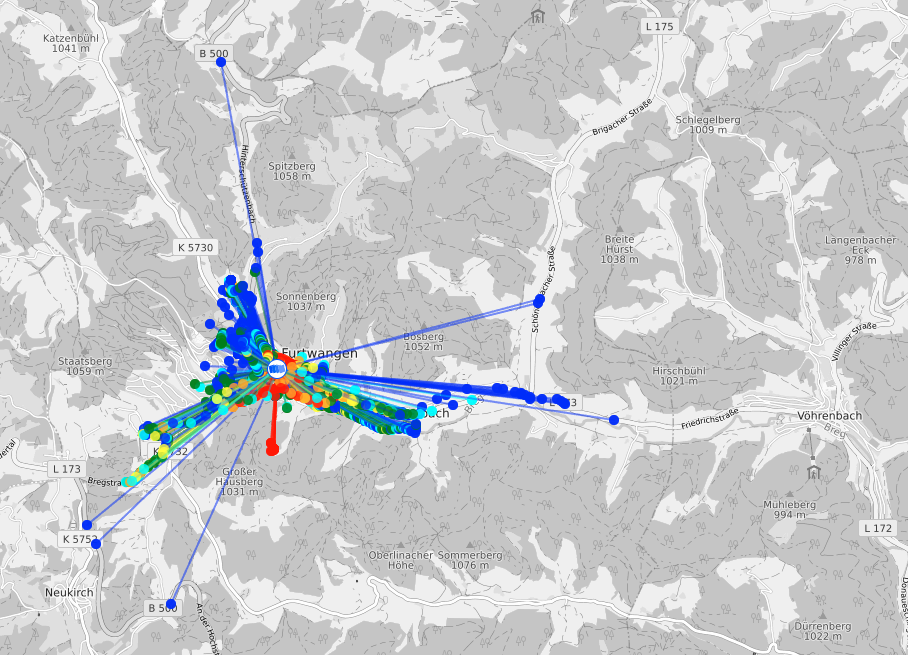
\includegraphics[width=1\textwidth]{pictures/ttn-mapper/gateway-ranges/c_building_gw_range.png}
    \caption{
        Map of some \ac{TTNM} data points taken from the \ac{LoRaWAN} gateway deployed on top of the C building.
        The slightly smaller range compared to \cref{pic:ghb_mikrotik_gw_range} is evident.
        The maximum range, however, is still \SI{4.3}{\kilo\meter} which is the rightmost blue point in the direction of Vöhrenbach.
    }\label{pic:c_building_gw_range}
\end{figure}

\Cref{pic:c_building_gw_range} shows the range of the \ac{HFU} C building gateway.
Clearly visible is the slightly smaller range compared to \cref{pic:ghb_mikrotik_gw_range}.
The maximum range recorded for this gateway is \SI{4.3}{\kilo\meter}, which is the rightmost blue point in the direction of Vöhrenbach again.

Installing the gateway on the roof of the \ac{HFU} C building was rather easy since accessing the roof is not difficult.
The cable of the antenna had to be pulled through a small conduit in the outer wall.
Afterwards, it could be connected to the \ac{LoRaWAN} gateway located inside a small crawl space.

Getting the network backhaul up and running wasn't as straightforward, though.
There were no spare Ethernet ports available in the crawl space.
However, there was a spare fiber optic cable run that was not in use at the moment.
Using two media converters, the fiber optic cable was converted to Ethernet and connected to the \ac{HFU} network one story below the roof.

\subsection{\acf{ASH}}

Installing the \ac{LoRaWAN} gateway on the roof of the \ac{ASH} building was an arduous task, but it was worth it.
The roof is difficult to access, and the gateway had to be installed on top of an antenna mast.

Getting a backhaul connection was rather easy, since a \ac{PoE} switch was available in the server room just beneath the roof.

However, the range, as shown in \cref{pic:ash_gw_range}, is very good and covers almost the entire Furtwangen area.
It is similar to the coverage of the \ac{GHB} building, since the \ac{ASH} building is also a multi-story building on a hill.

\begin{figure}[htbp]
    \centering
    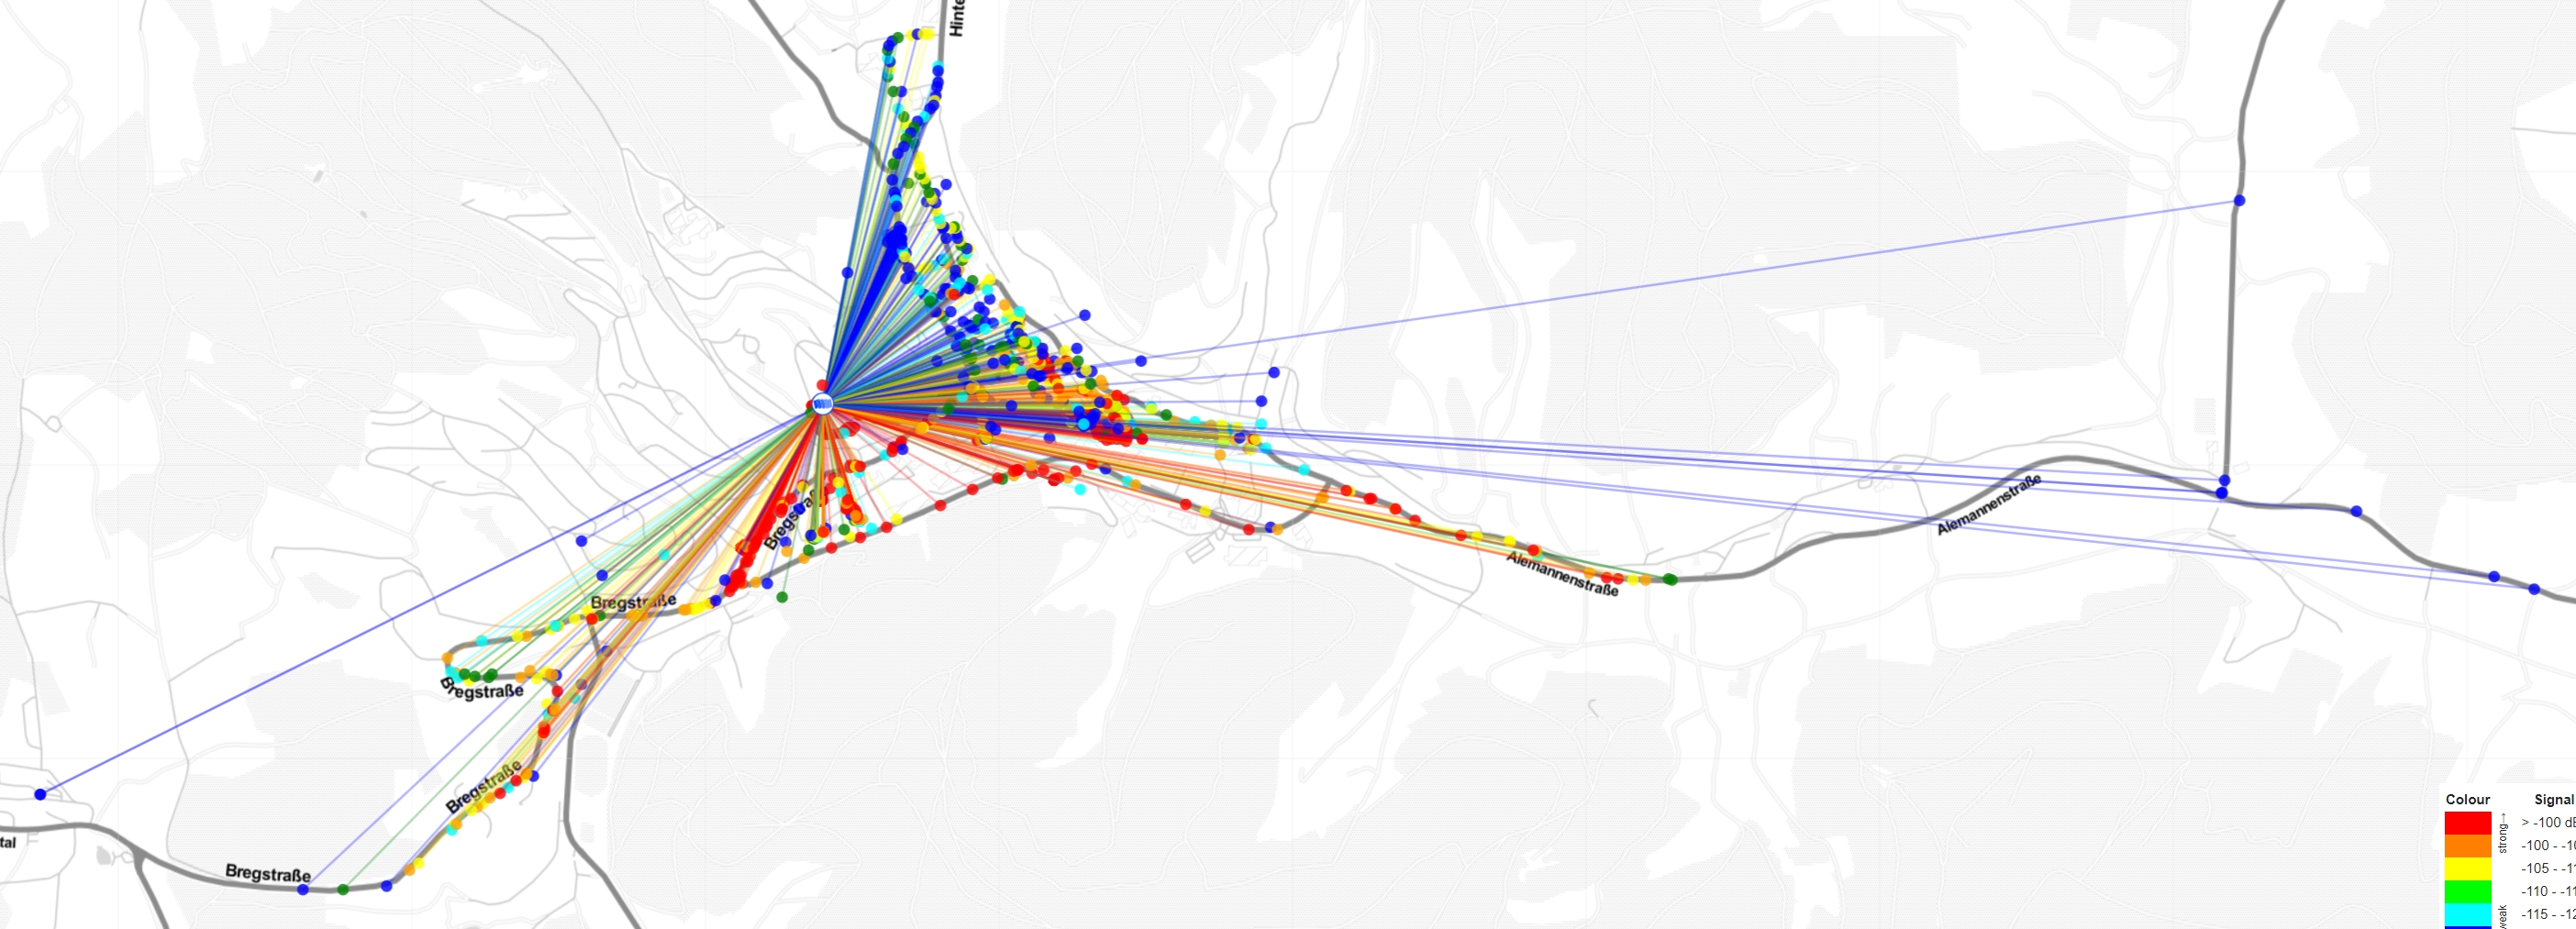
\includegraphics[width=1\textwidth]{pictures/ttn-mapper/gateway-ranges/ash_gw_range.jpg}
    \caption{
        Map of some \ac{TTNM} data points taken from the \ac{LoRaWAN} gateway deployed on the roof of the \ac{ASH} building.
        It has a good range into most parts of the Furtwangen area.
    }\label{pic:ash_gw_range}
\end{figure}

The longest range recorded from the \ac{ASH} building thus far is around \SI{4.8}{\kilo\meter} which is the blue point on the right of \cref{pic:ash_gw_range}.

\subsection{\emph{DL0FIS} amateur radio club station}

While the location of the \ac{LoRaWAN} on top of a hill between Furtwangen and Gütenbach should have made for very good coverage, the reality looks different.

\begin{figure}[htbp]
    \centering
    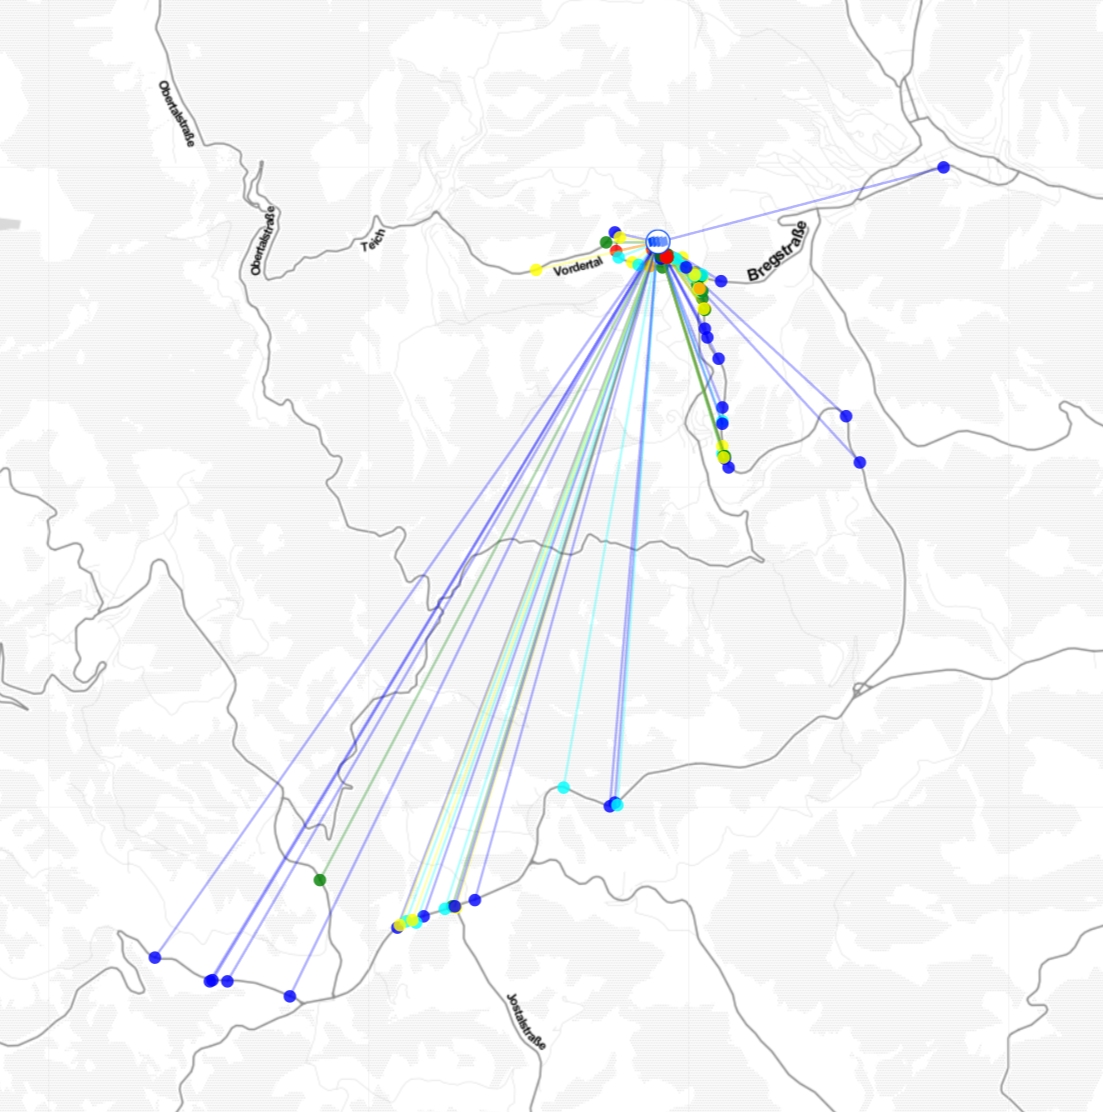
\includegraphics[width=1\textwidth]{pictures/ttn-mapper/gateway-ranges/dl0fis_gw_range.jpg}
    \caption{
        Map of some \ac{TTNM} data points taken from the \ac{LoRaWAN} gateway deployed on the roof of the \emph{DL0FIS} clubhouse.
        While the range is not consistent in every direction due to the hills and mountains in the area, the longest range of around \SI{8.8}{\kilo\meter} is still very good.
        The range to the city of Furtwangen is almost nonexistent due to the hills in the way.
    }\label{pic:dl0fis_gw_range}
\end{figure}

\Cref{pic:dl0fis_gw_range} shows the coverage of the \ac{LoRaWAN} gateway deployed on the roof of the \emph{DL0FIS} clubhouse.
The longest range measured was one data point in the south with a distance of \SI{8.8}{\kilo\meter}.
The gateway, up until now, wasn't of much use in the scope of this thesis though, since the hill between the Neueck clubhouse and the city of Furtwangen blocks most of the signal.

Getting a backhaul connection to the \ac{LoRaWAN} gateway was easy since the clubhouse is equipped with a stable internet connection.
The gateway could thus be connected using Ethernet.

\subsection{\acs{HFU} O building}\label{subsec:conclusion-hfu-o-building}

Another possible location that was not mentioned in \cref{sec:gateway-locations} was the \ac{HFU} O building.
Located in the northern part of Furtwangen, it is a multi-story building that used to be a hospital.
Since the \ac{HFU} is only a tenant there, permission was needed from the building owner to install the gateway.
Fortunately, the owner, Mr.\ Odin Jäger, was very cooperative and allowed the gateway to be installed.

Unfortunately, it was not as easy to get a network connection and power on the roof as it was in the other buildings, so no gateway has been installed there yet.

\subsection{Factory building of the \emph{E. Wehrle GmbH} company}\label{subsec:factory-building-of-the-e-wehrle-company}

Although not considered at the beginning of this thesis, during the first weeks of data collection with \ac{GPS} trackers in Furtwangen, a gateway appeared in the \ac{TTN} packet metadata that had no location entered.
After some investigation, it turned out that the gateway was located on the roof of the factory building of the \emph{E. Wehrle GmbH} company in the southwestern part of Furtwangen.
After contacting the company, Tom Lehmann, an external consultant for the company working at \emph{Netzint GmbH}, was very cooperative and entered its location into the \ac{TTN} console.
This allowed the gateway to be displayed on the \ac{TTNM} map and for its data to also be considered in the \ac{TTNL} calculations.

The \emph{E. Wehrle GmbH} company is a manufacturer of (among other products) smart metering sensors.
Alongside other protocols, they also use \ac{LoRaWAN} for some of their products~\cite{e_wehrle_gmbh_wecount-s_nodate}.

\section{Collected data in Furtwangen on \acl{TTNM}}\label{sec:collected-data-in-furtwangen-on-ttnm}

\subsection{\acl{TTNM} heatmap view after additional data collection}\label{sec:ttm_heatmap_after}

During the course of this thesis, additional data was collected using the \ac{LoRaWAN} \ac{GPS} trackers mentioned in \cref{subsec:used-lora-nodes}.
This lead to a denser data coverage of \acl{TTNM} in the Furtwangen area.

\begin{figure}[htbp]
    \centering
    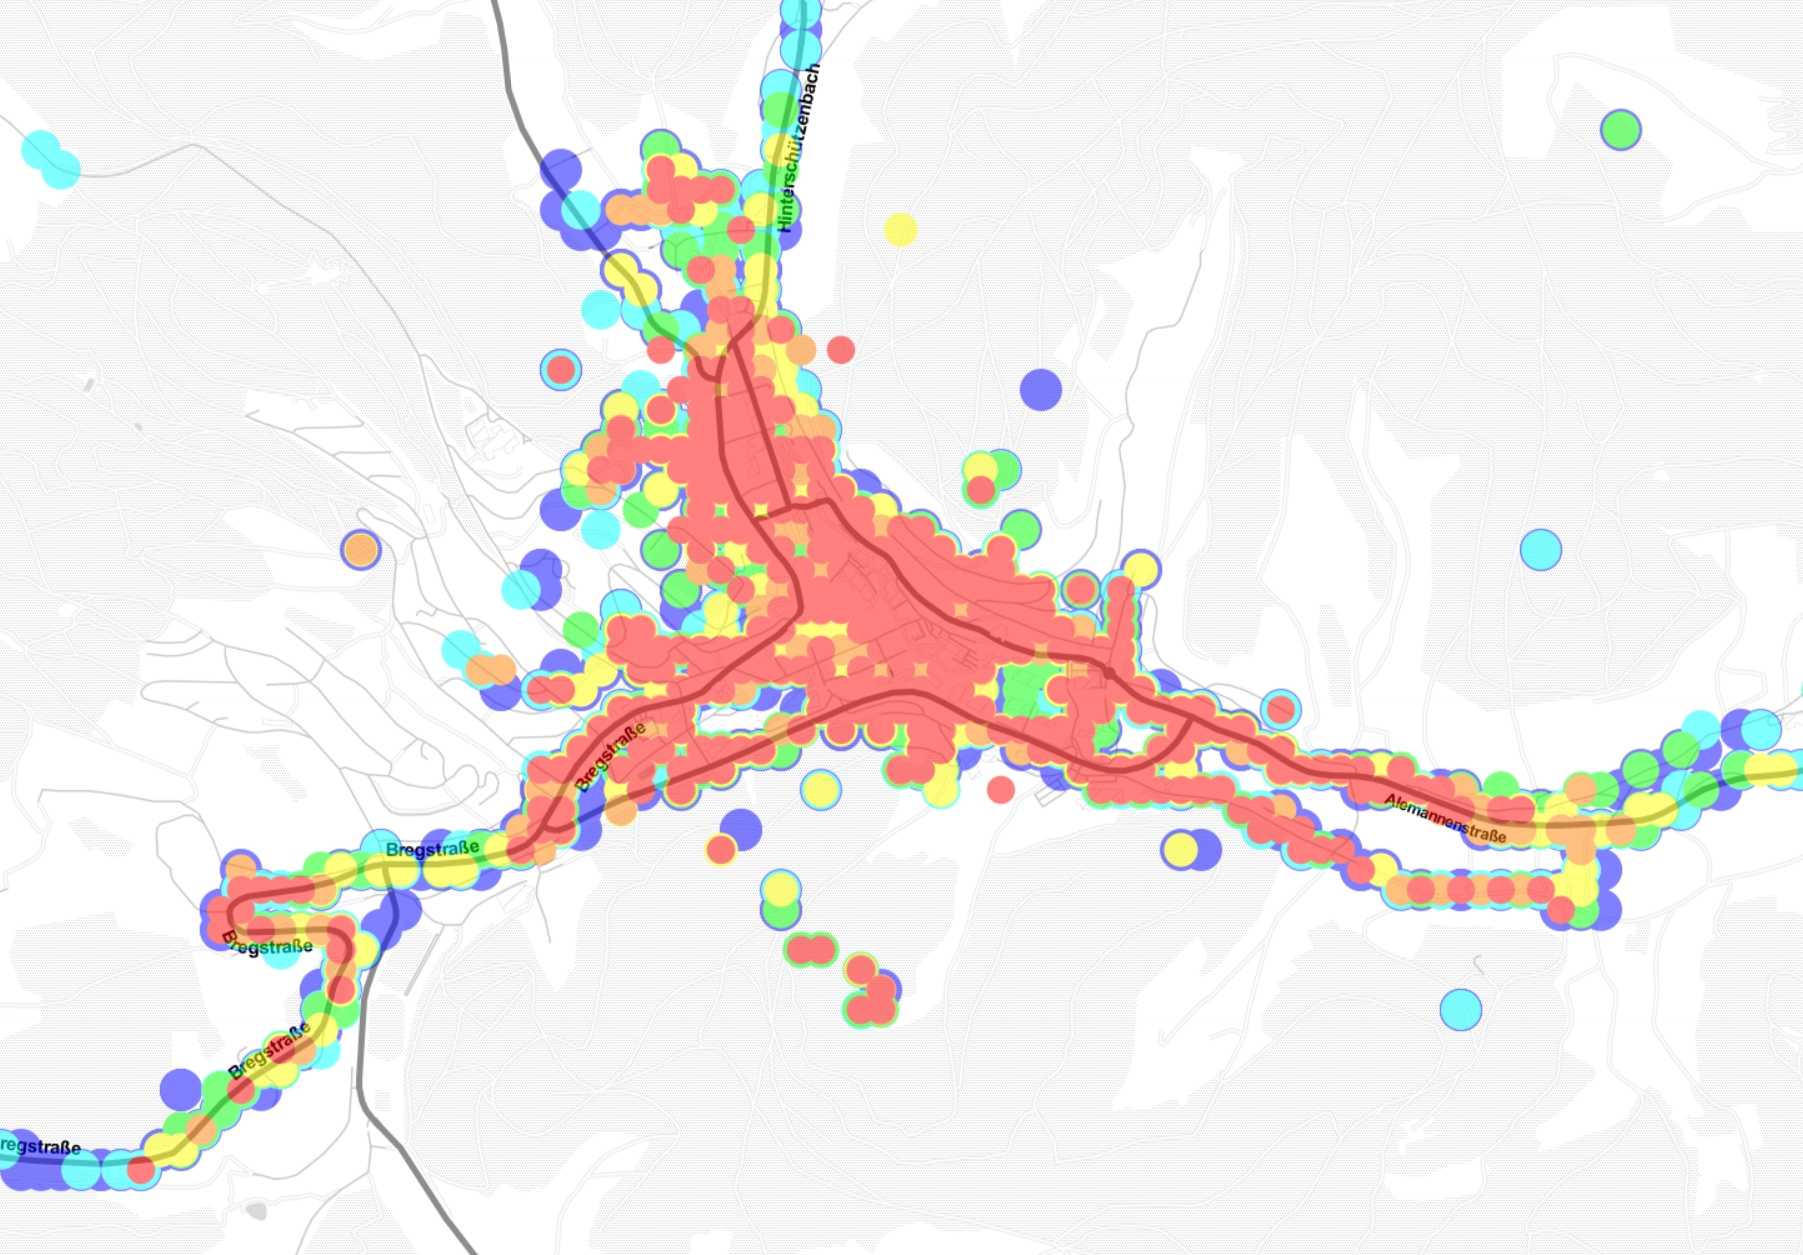
\includegraphics[width=0.7\textwidth]{pictures/ttn-mapper/ttnm_heatmap_after_data_collection.jpg}
    \caption{
        View of the \ac{TTNM} heatmap view after data collection during this thesis, from the 21st of June 2023.
        Compared to \cref{pic:ttnm-before-data-collection}, the coverage is better.
        This is due to the fact that several \ac{LoRaWAN} gateways were deployed during this thesis as well as the additional data collection performed with \ac{LoRaWAN} \ac{GPS} trackers.
    }\label{pic:ttnm-heatmap-after-data-collection}
\end{figure}

\Cref{pic:ttnm-heatmap-after-data-collection} shows a view of the \ac{TTNM} heatmap after the additional data collection that was done during this thesis.
The much redder color of the map is visible, meaning that the signal strength in these areas is stronger than before.

While there are still some blank spots, these are mostly due to the fact that these areas were not visited by \ac{GPS} trackers during the data collection in this thesis.

\section{Comparison of Geolocation Methods}

This section will compare the different geolocation methods that were used in this thesis.

\subsection{Multilateration}\label{subsec:conclusion-multilateration}

\subsubsection{\acf{RSSI}}

\Cref{lst:sql-calculate-correlation-coefficient} shows a \ac{SQL} query that was used to calculate the correlation coefficient between \ac{RSS} values and their associated distances for a single gateway.
Its purpose is to show how much the \ac{RSS} values correlate with the distance from the end device to the gateway.

\begin{lstlisting}[
    language=SQL,
    float,
    caption={
        \ac{SQL} query used to calculate the correlation coefficient between \ac{RSS} values and associated distances for a single gateway.
        This query was also generated by \emph{Bing AI} and adjusted to fit the the application's needs.
        The \lstinline|CORR| function was used to calculate the correlation coefficient over the gateway's data points.
    },
    label={lst:sql-calculate-correlation-coefficient}
]
WITH gateway_data AS (
    SELECT
        gateway.latitude AS gateway_latitude,
        gateway.longitude AS gateway_longitude,
        deviceGPSDatapoint.latitude AS datapoint_latitude,
        deviceGPSDatapoint.longitude AS datapoint_longitude,
        ttnMapperDatapoint.rssi AS rssi
    FROM
        "Gateway" gateway
        JOIN "TtnMapperDatapoint" ttnMapperDatapoint ON gateway."gatewayId" = ttnMapperDatapoint."gatewayId"
        JOIN "DeviceGPSDatapoint" deviceGPSDatapoint ON ttnMapperDatapoint."deviceGPSDatapointId" = deviceGPSDatapoint.id
    WHERE
        gateway."gatewayId" = 'hfu-lr8-001'
),
distance_data AS (
    SELECT
        *,
        ST_DistanceSphere(
            ST_MakePoint(gateway_longitude, gateway_latitude),
            ST_MakePoint(datapoint_longitude, datapoint_latitude)
        ) AS distance
    FROM
        gateway_data
),
stats_data AS (
    SELECT
        CORR(distance, rssi) AS correlation_coefficient,
		COUNT(*) AS datapoint_count
    FROM
        distance_data
)
SELECT * FROM stats_data;
\end{lstlisting}

The result for a data set of about \num{10000} collected ttnMapperDatapoints from the \ac{GHB} MikroTik gateway is roughly equal to \num{-0.261}, indicating a medium to weak negative correlation between the \ac{RSS} values and the distance to the gateway.
Other gateways show similar results.

This means that, in general, \ac{RSS} values alone are not a good indicator for measuring distances.
Still, this chapter will provide an overview over the techniques used during this thesis to estimate the position of a device based on \ac{RSS} values in two different ways.

\paragraph{Accuracy of \acs{RSSI}-based multilateration with a fixed \acs{RSS} to range function}\label{subsubsec:conclusion-rssi-fixed-scale}

As shown in \cref{sec:fixed-rssi-to-range-scale-impl}, a fixed \ac{RSS} to range mapping was implemented in the frontend first.
In general, the accuracy of using such a fixed \ac{RSSI} to range mapping was poor.

\begin{figure}[htbp]
    \centering
    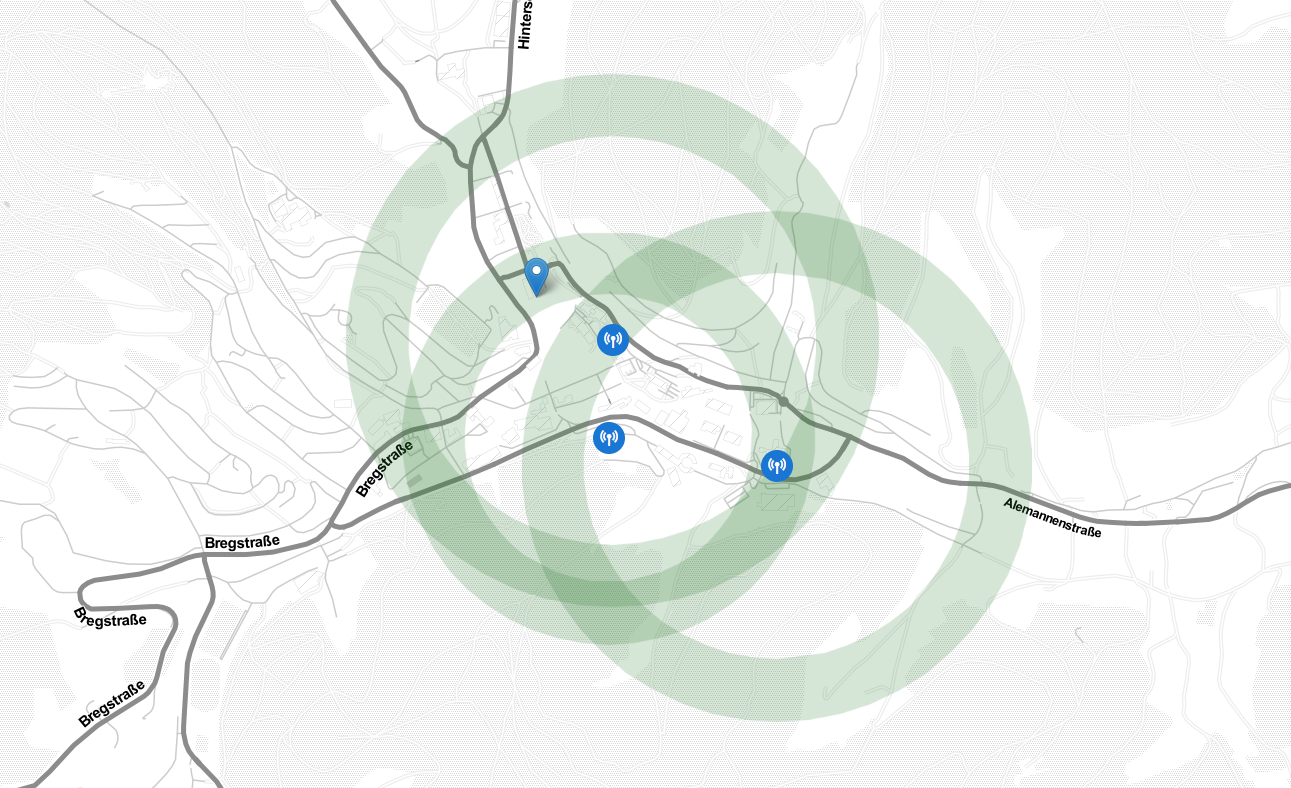
\includegraphics[width=0.8\textwidth]{pictures/ttn-locator/frontend/multilateration/rssi_range_multilateration_bad_example.png}
    \caption{
        Example of a multilateration with three gateways using a fixed \ac{RSSI} to range mapping.
        It can be seen that the estimated position, where the three green annuli intersect, is quite far away from the actual position (blue pin) of the device.
        The width of the annuli is an arbitrary value of \SI{100}{\meter} in this case.
        The value can be changed in the frontend to test various error margins.
        The annuli are drawn using Leaflet's ability to render GeoJSON.
    }\label{pic:bad-rssi-to-range-multilateration-example}
\end{figure}

\Cref{pic:bad-rssi-to-range-multilateration-example} shows an example of a multilateration with a fixed \ac{RSSI} to range mapping where the result is not at all accurate.

\paragraph{Accuracy of \acs{RSSI}-based multilateration with linear regression per gateway}\label{subsubsec:conclusion-rssi-linear-regression}

As mentioned in \cref{subsubsec:per-gateway-rssi-to-range-scale}, another idea was to use linear regression to map \ac{RSS} values to ranges for each gateway.
This approach considers gateway-specific parameters such as position and gateway antenna gain.
However, it cannot consider \ac{MPP} effects as well as end device antenna gain.

\begin{figure}[htbp]
    \centering
    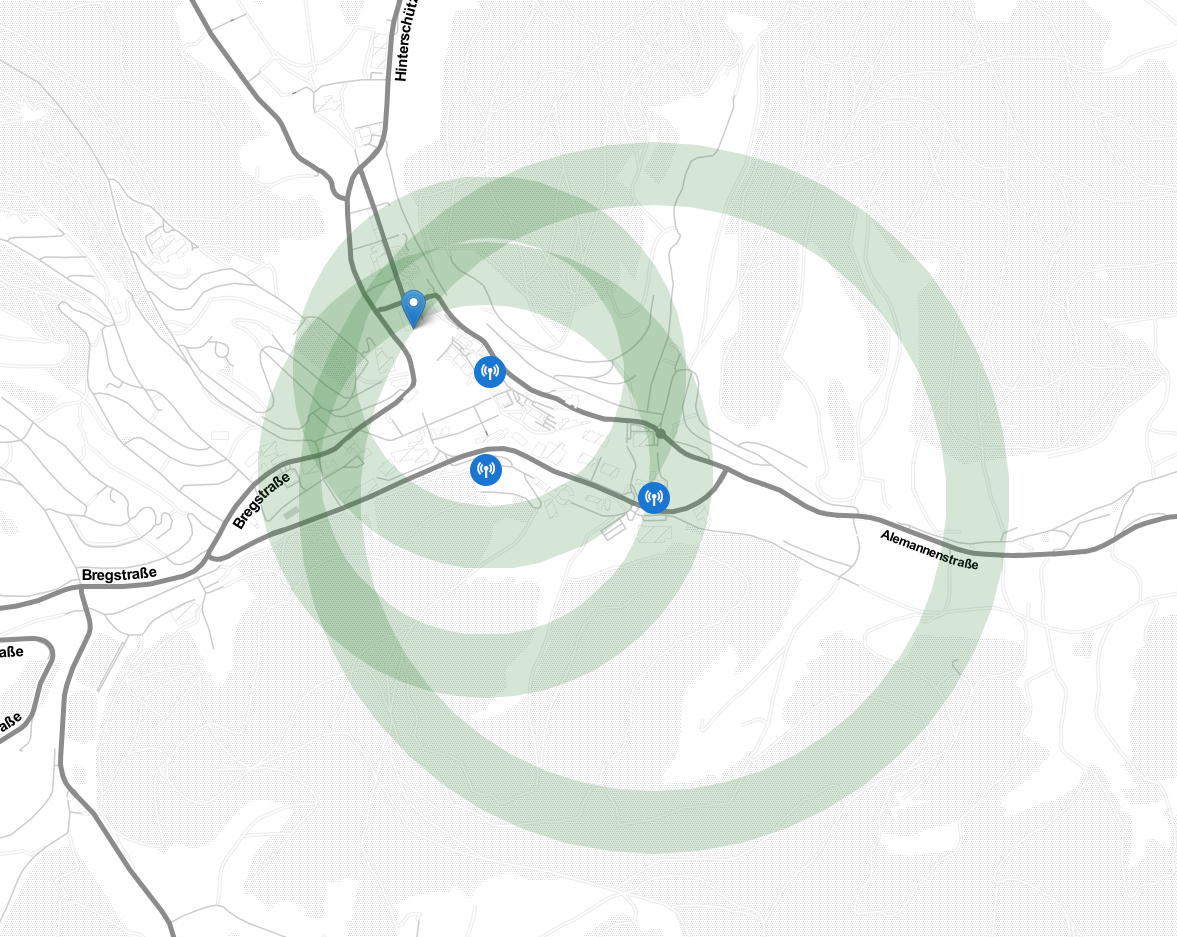
\includegraphics[width=0.8\textwidth]{pictures/ttn-locator/frontend/multilateration/rssi_range_multilateration_regression_example.png}
    \caption{
        Example of a multilateration with three gateways using a linear regression based \ac{RSSI} to range mapping per gateway.
        It uses the same base data point as seen in \cref{pic:bad-rssi-to-range-multilateration-example}.
        The estimated position, where the three green annuli intersect, is more accurate compared to the fixed range mapping.
        The width of the annuli is, again, an arbitrary value of \SI{100}{\meter}.
    }\label{pic:rssi-to-range-multilateration-example-with-linear-regression}
\end{figure}

\Cref{pic:rssi-to-range-multilateration-example-with-linear-regression} shows an example of the same data point as in \cref{pic:bad-rssi-to-range-multilateration-example} but with such a linear regression model that determines a mapping of \ac{RSS} values to ranges for each gateway.
The example shows that the resulting position estimation where the three annuli intersect is better than before.
However, since the linear regression model cannot account for \ac{MPP} effects either, the results still typically deviate from the actual position by a few hundred meters.

\paragraph{Conclusion}

As was explained in \cref{sec:multipath-propagation}, \acl{MPP} effects can cause the \ac{RSS} values to fluctuate heavily.
In addition, as explained in \cref{sec:rssi}, different antennas on gateways and end devices can cause different \ac{RSS} values to be measured for the same distance due to different antenna gains.

This makes multilateration with \ac{RSS} values as the only input data inaccurate.
Even when using a linear regression model to generate a mapping of \ac{RSS} values to ranges for each gateway, the results were often inaccurate.

\subsubsection{\acf{ToA}}\label{subsec:conclusion-toa-tdoa}

\Cref{subsec:toa-based-multilateration-implementation} mentioned the fact that using timestamps from a \ac{LoRaWAN} gateway to determine the range to the end device is too inaccurate to be used for \ac{ToA}-based geolocation.

In addition to the fact that timestamps arrive at \ac{TTN} with unrealistic offsets due to missing time synchronization, another factor has to be considered.
The device timestamps arrive at \ac{TTN} in a format such as \texttt{2023-06-23T15:11:11.678179Z}.
The six decimal places after the seconds mean that the timestamp is accurate to \SI{1}{\micro\second}.
\Cref{eq:toa-accuracy-ttn-microseconds} shows that when using microseconds to calculate the distance to a \ac{LoRaWAN} gateway based on the speed of light, a maximum accuracy of \SI{300}{\meter} can be achieved.

\begin{equation}\label{eq:toa-accuracy-ttn-microseconds}
    \text{ToA\,accuracy}_{\si{\micro\second}} = \frac{299792458 \frac{\si{\meter}}{\si{\second}}}{10^6} \approx 300 \si{\meter}
\end{equation}

\Cref{eq:toa-accuracy-ttn-nanoseconds} shows that using nanoseconds, a much better accuracy of \SI{0.3}{\meter} could be achieved.

\begin{equation}\label{eq:toa-accuracy-ttn-nanoseconds}
    \text{ToA\,accuracy}_{\si{\nano\second}} = \frac{299792458 \frac{\si{\meter}}{\si{\second}}}{10^9} \approx 0.3 \si{\meter}
\end{equation}

Solving this problem on the scope of the entire \ac{TTN} \ac{LoRaWAN} network is not feasible because it would require synchronizing the clocks of all gateways in the network with \ac{GPS} receivers.
However, if one were to deploy a \ac{LoRaWAN} network in a smaller area where control over every reachable gateway is realistic, this would be a possible solution.
If every gateway in the network is time-synchronized, \ac{ToA} could be used for geolocation.

\subsection{Fingerprinting}

% TODO: describe how this worked and how it could be improved (worked pretty okay but has only limited accuracy)

\Cref{fig:fingerprinting-map-example-only-center} already showed an example where the center of matching filtered data points was taken as the estimated position, along with an arbitrary radius to show the associated uncertainty.

\begin{figure}[htbp]
    \centering
    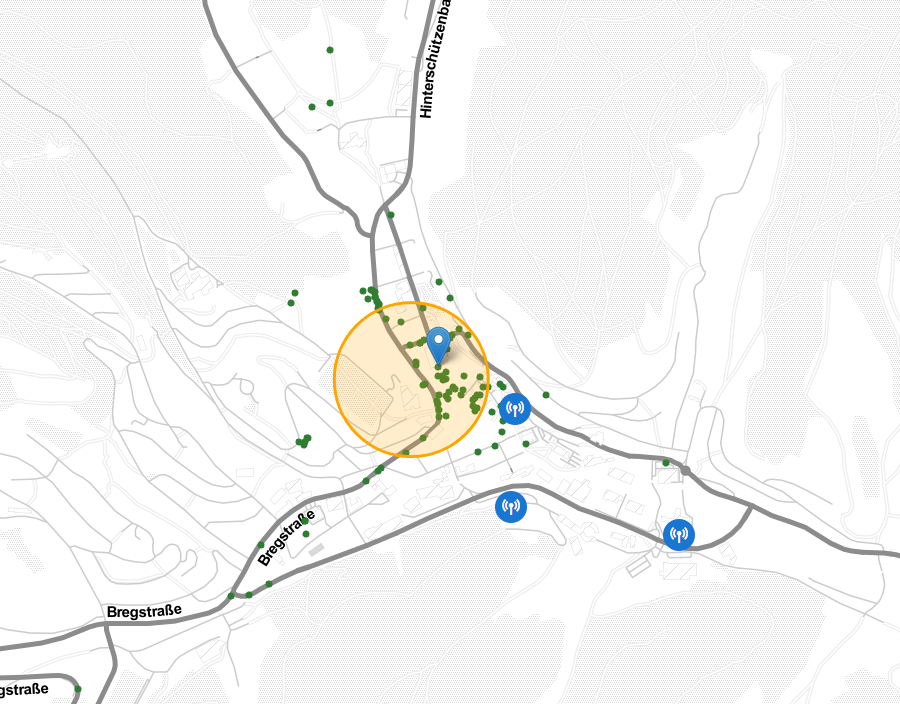
\includegraphics[width=0.6\textwidth]{pictures/ttn-locator/frontend/fingerprinting/rssi_similarity_map_example_dynamic_radius.png}
    \caption{
        Example for a fingerprinting result map generated by \ac{TTNL}.
        The blue pin shows the actual position of the device.
        The yellow circle shows the estimated position that \ac{TTNL} calculated out of the center of the matching data points.
        The radius is determined by having half of the matched points fit inside it.
    }\label{fig:fingerprinting-map-example-dynamic-radius}
\end{figure}

On the other hand, \cref{fig:fingerprinting-map-example-dynamic-radius} shows an approach where the error radius is not arbitrary, but is calculated based on fitting half the matched points inside the circle.
This usually results in a larger error radius (low precision), but a higher rate of actually containing the actual position (high accuracy).

% TODO: mention the potential of using machine learning to improve the fingerprinting method

% TODO: mention that snr and sf could also be used for fingerprinting

In comparison to the multilateration approach, the fingerprinting approach is not very scalable.
It requires considerable manual work to create a fingerprint database for a certain area.
This makes it only feasible for smaller, contained areas and rather unusable for larger-scale geolocation such as in a whole city or state.

\section{Comparison of findings with existing work}

Several of the approaches found in \cref{sec:related-work} have better success in locating endpoints than the work in this thesis.
This could be due to the fact that these approaches use more tightly controlled environments, such as having \ac{LoS} between the end device and the gateways.
Nevertheless, the work in this thesis was successful in terms of rough geolocation.

The hardware deployments in this thesis were less focused on getting good geolocation results and more focused on getting a large amount of data from a wide variety of devices and gateways.
This variety is also the case in real-world \ac{IoT} deployments.
As far as \ac{LoRaWAN} coverage in the city of Furtwangen is concerned, this can be considered a success.
As was shown in \cref{sec:gateway-locations-conclusions}, \ac{TTNM} now looks a lot more complete than it did before the work during this thesis.

\section{Outlook}

This section will provide an outlook on possible future work that could be done in relation to this thesis.

\subsection{Improving the \acf{TTNL} software}

This section will mention some ideas on how to improve the \ac{TTNL} software.

\subsubsection{Automatically detecting moved gateways}

Although rare, it is possible for a \ac{LoRaWAN} gateway to be moved to a different location, or to have a different location set in the \ac{TTNL} console than it had before.
Since the \ac{TTNL} software currently updates the gateway location after each \ac{TTNM} data collection run, it is possible for a gateway to be moved and not be detected by the \ac{TTNL} software.
This can lead to inaccurate geolocation results if gateways are actually moved.

A change should be made to the \ac{TTNL} backend where, on detection of a gateway moving further than a certain distance, each TtnMapperDatapoint associated with it is deleted to avoid the usage of false data in the calculations.

\ac{TTNM} seems to do a similar thing based on the section ``My results were showing on the map before, but is gone now.'' in their FAQ~\cite{ttn_mapper_faq_nodate}.
However, as far as the duration of this thesis is concerned, this was not observed.
The gateway that is now deployed on the roof of the \emph{DL0FIS} clubhouse once was located on the \ac{HFU} B building, but was then moved to its final location.

\subsubsection{Remove dependency on \acl{TTNM}}

Since this thesis is largely based on \ac{TTNM}, it would be beneficial to remove the dependency on it.
Should \ac{TTNM} ever be discontinued, the \ac{TTNL} software would no longer be able to function in its current state.
A taste of such a situation was already experienced during the development of this thesis, when the \ac{TTNM} \ac{API} was down for several hours one day during the development phase.

To remove the dependency on \ac{TTNM}, the \ac{TTNL} software could be extended to include its own \ac{REST} endpoints, providing the same ability to receive data directly from \ac{TTN} as \ac{TTNM}.
This would enable the \ac{TTNL} software to function without \ac{TTNM} and would also allow for more flexibility in data collection in the future.

\subsubsection{Better sharing of type definitions between Frontend and Backend}\label{subsubsec:outlook-sharing-type-definitions}

Because the frontend and backend were split up into two separate repositories, some \ac{TS} type definitions had to be duplicated.
This resulted in some manual work when changing the type definitions, as changes had to be applied to both repositories.
In the future, this could be improved in several ways.
For example, the frontend and backend could be merged into a single repository.
The type definitions could also be moved to a separate repository that is used as a dependency in both the frontend and backend repositories.

\subsubsection{Choice of technologies}

This section will critically reflect on the choice of technologies used in this thesis as well as mention some alternatives.

\paragraph{Full Stack Frameworks (SvelteKit, Nuxt.js)}

As an alternative to the approach described in \cref{subsubsec:outlook-sharing-type-definitions}, the entire project could have been written using a full-stack framework such as SvelteKit or Nuxt.js.
This would also have allowed the entire project to be in a single repository, which would have made sharing type definitions easier.

However, this would also have meant a much tighter coupling of the \ac{TTNL} frontend and backend.
As a result, it would no longer be possible to deploy the \ac{TTNL} frontend and backend services separately as Docker containers, since the entire project would have to be deployed as a single Docker container.

\paragraph{Prisma}

While Prisma enables the developer to write type safe \ac{DB} queries using \ac{TS}, it does not support all possible queries (yet).
Some advanced queries, such as the one shown in \cref{lst:sql-remove-outliers}, had to be written by hand using \ac{SQL} and executed using Prisma's \lstinline|$executeRaw| method.
There were several such cases in this thesis, which is why it might have been more suitable to not use Prisma at all and instead use \ac{SQL} in a more direct way.

However, the ability of Prisma to generate migrations from a schema and its type safety were still useful features that made it worth using.
Prisma's schema file also acts as indirect documentation of the \ac{DB} structure, which is useful for other developers that might want to contribute to the project.

An alternative to Prisma would have been PgTyped, which is a library that can generate typesafe \ac{SQL} queries from \ac{TS} type definitions~\cite{salakh_pgtyped_2023}.

Another alternative would have been to use \emph{GraphQL} instead of \ac{HTTP} \ac{REST} calls.
GraphQL is a method for writing \ac{API} queries that lets the client specify which data it wants to receive from the server~\cite{graphql_foundation_graphql_2023}.
It uses a syntax to modify and request data that is similar to \ac{JSON}.
In doing so, GraphQL also ships its own type system that can be used to generate type definitions for the frontend.

\subsubsection{Recognizing moving gateways}

Currently, the backend of the \ac{TTNL} software cannot recognize if a gateway has moved its position since the last time it was captured.
This can lead to problems when the gateway is moved to a different location, as the software will still use the old location for the gateway and assumes that its previous data
points were captured at the same location.

\begin{figure}[htbp]
    \centering
    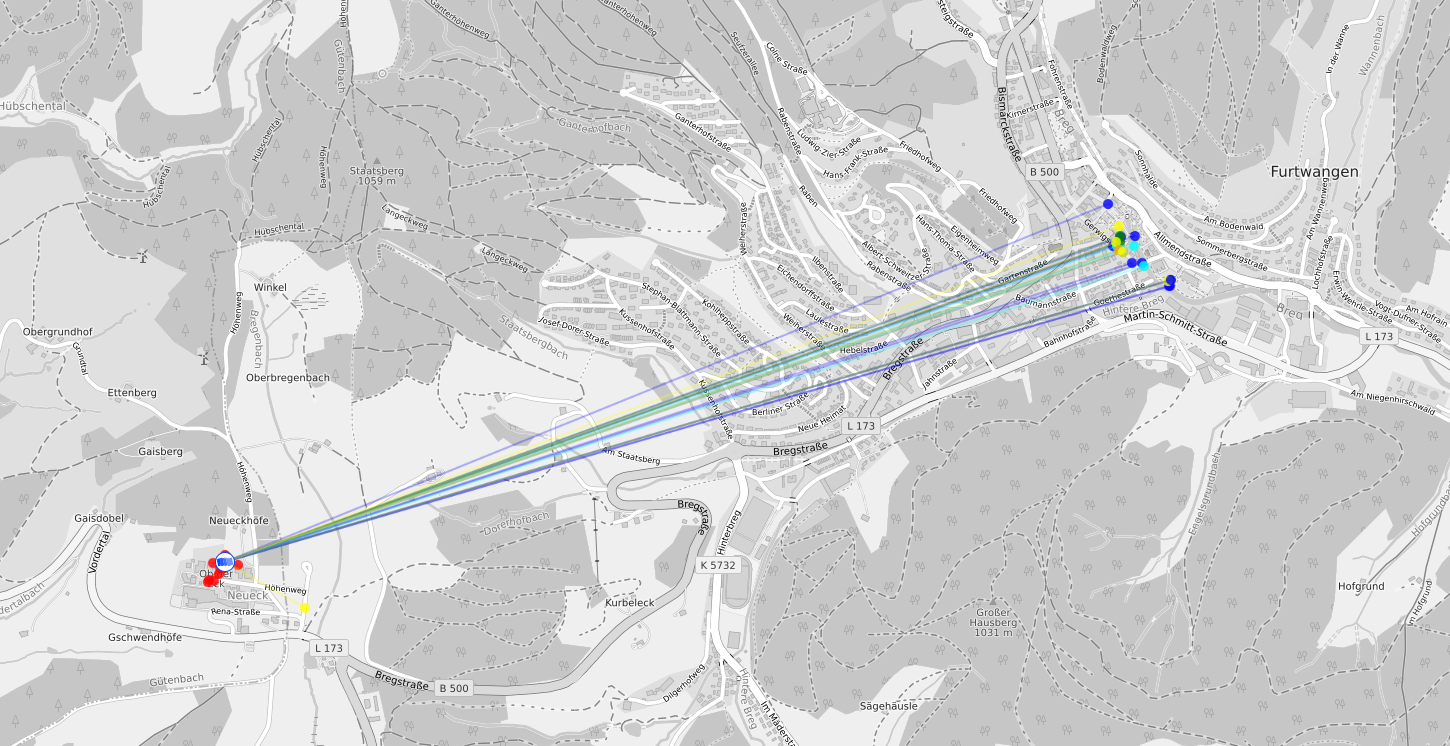
\includegraphics[width=0.9\textwidth]{pictures/ttn-mapper/moved_gateway_example.png}
    \caption{
        Example of false data being displayed on a \acl{TTNM} map due to a gateway being moved.
        The gateway placed on the right is the one on the roof of the \emph{DL0FIS} clubhouse.
        The data points on the right are from before the gateway was moved there when it was still on the roof of the \ac{HFU} B building.
    }\label{pic:gateway-moved-example}
\end{figure}

\Cref{pic:gateway-moved-example} shows an example where this happened in \ac{TTNM}.
\ac{TTNL} could be improved by adding a feature that recognizes if a gateway has moved and then deletes all data points that were captured at the old location of the gateway.

\subsection{Projects made possible due to better \acs{LoRaWAN} coverage in Furtwangen}

As there are now several new \ac{LoRaWAN} gateways in Furtwangen, there are several projects that can be done in the future that would not have been possible before without installing such gateways by oneself.

This section will list some of these projects and describe how they could be implemented.

\subsubsection{Measuring the water level of the Breg river}

One of the \ac{LoRaWAN} nodes ordered as part of this thesis is a \emph{Milesight EM310-UDL}, an ultrasonic distance/level sensor.
As the \ac{LoRaWAN} network coverage of Furtwangen is now adequate, it would be possible to use this sensor to measure the water level of the Breg river flowing through the vicinity of the \ac{HFU}.
This would allow for a more accurate prediction of the water level of the Breg river, which might in turn allow for a more accurate prediction of the water level of the Danube river.
Installing this \ac{LoRaWAN} node as well as connecting it to \ac{TTN} and adding an \acf{AS} to it to allow monitoring of the water level of the Breg river would be a good future project for students of the \ac{HFU}, enabled by the gateways placed during this thesis.

\subsubsection{Measuring soil moisture and environmental conditions in the Furtwangen city park}

The same semester, Samuel Kasper, a student of the \ac{DM} faculty of the \ac{HFU} wrote his bachelor thesis about measuring the humidity as well as the temperature of the soil to monitor plants and crop growth.
The installation of \ac{LoRaWAN} gateways in the city of Furtwangen helped him in this regard, as he did not have to install his own gateways and instead could use the now existing infrastructure in the city.

\subsubsection{Monitoring of Gateways}

Another possible project would be an application that monitors the gateways and checks if they are still online.
Such a project could be realized with software like \emph{Node-RED}.~\cite{openjs_foundation_node-red_nodate}

\subsection{Further research}

\subsubsection{Improving timestamp accuracy for \acf{ToA} geolocation method}

As mentioned in \cref{subsec:conclusion-toa-tdoa}, the accuracy of the \ac{ToA} method could be greatly improved if nanosecond level timestamps were available.
Unfortunately, \ac{TTN} does not provide nanosecond level timestamps for the packets received by the \ac{LoRaWAN} gateways.
To solve this problem, a \ac{LNS} would need to be set up that has the ability to do that.

In addition, \ac{LoRaWAN} gateways would need to be time synchronized to achieve the best possible accuracy.
The latter problem could be solved by using \ac{GPS} receivers to synchronize the gateways.
While some gateways have \ac{GPS} built-in receivers, most do not.
For example, the \emph{Dragino DLOS8N} that was used twice during this thesis has a \ac{GPS} built-in receiver~\cite{dragino_technology_co_ltd_dlos8n_2023}, but none of the others do.

In any case, using the \ac{ToA} method would require more specific hardware than what most of the \ac{TTN} community network currently uses.
This makes it unsuitable for widespread use on that particular network.

\subsubsection{Using \acf{ML} to improve the fingerprinting method}

There are several \ac{ML} methods that could be used to improve the fingerprinting method.
For example, \ac{kNN} could be used to determine the location of a node based on the \ac{RSS} values of the surrounding gateways~\cite{anagnostopoulos_reproducible_2019}.

\subsubsection{Also use \ac{SF} and \ac{SNR} values for fingerprinting}

As mentioned in \cref{sec:sf-snr-correlation}, the \ac{SF} used by the end device has an influence on the \ac{SNR} values at which a signal can still be detected.
This means that the \ac{SF} and \ac{SNR} values used by the end device could also be used to more accurately determine the location of the end device.
Since the \ac{TTN} data frames include this information, it could be used to improve the fingerprinting method.

A disadvantage of this approach would be that it would require more data to be collected, since the number of possible variables per captured gateway would increase from 1 (\ac{RSSI}) to 3 (\ac{RSSI}, \ac{SF}, \ac{SNR}).

\subsubsection{Using a Kalman filter to improve localization of devices known to be stationary}

% TODO: Descrbe this?

\subsubsection{Gateway on the roof of the \acs{HFU} O building}

As was mentioned in \cref{subsec:conclusion-hfu-o-building}, the roof of the O building would make another good location for a \ac{LoRaWAN} gateway.
The permission by the building's owner was granted.
The problem that would need to be solved is getting a network connection as well as power to the roof of the building.

Another option that would only require getting power to the roof is to use a \ac{LoRaWAN} gateway that has a \ac{LTE} backhaul connection.
However, getting a \ac{PoE} connection to the roof of the building would still be preferable due to its stability.

\subsubsection{Meshing / repeating of \acs{LoRaWAN} gateways}

While \ac{LoRa} allows for communication between any sort of \ac{LoRa} device, be it end device or gateway, \ac{LoRaWAN} does not.
Theoretically, a gateway to gateway communcation in pure \ac{LoRa} is possible.
However, this behavior is not implemented in the \ac{LoRaWAN} protocol.

If this functionality could be implemented in the \ac{LoRaWAN} protocol, it would allow for a sort of meshed network of \ac{LoRaWAN} gateways.
Gateways acting as repeaters in such a network could forward \ac{LoRaWAN} packets without the need for a backhaul connection as mentioned in \cref{sec:gateways}.
Since the \ac{LoRaWAN} protocol doesn't provide this functionality yet, it would need to be tested with a custom implementation of gateway firmware first.

A \ac{LoRaWAN} related project that also uses \ac{LoRa} and can do meshing between devices is \emph{Meshtastic}~\cite{meshtastic_llc_meshtastic_2023}.
It uses hardware similar to the \ac{LoRaWAN} nodes used in this thesis to create a meshed network of devices that can communicate without the need for Internet access.

The German company \emph{Dryad Networks GmbH} also offers a proprietary meshed \ac{LoRaWAN} network~\cite{dryad_networks_gmbh_silvanet_2023}.
It is used to detect wildfires early using a network of \ac{LoRa} sensors that can send their data over meshed gateways to avoid the need for a backhaul connection for each gateway placed over large areas of forest.

Anton Petrov is going to write his master thesis about this topic in the coming winter semester of 2023/2024.
His thesis will also be supervised by Prof. Dr. Richard Zahoransky.

\subsubsection{Self-hosting of \acs{TTS} or \emph{ChirpStack}}

Another interesting project would be to self-host an instance of a \ac{LNS} like \ac{TTS} or \emph{ChirpStack} on \ac{HFU} infrastructure.
This would give students the opportunity to learn more about the inner workings of a \ac{LNS} and would also give the \ac{HFU} the ability to exert more control over the data collected by the \ac{LNS}.
Both of them are \ac{OSS} and can be self-hosted using Docker or Docker Compose.

\subsubsection{Privacy concerns}

Since the work in this thesis has shown that it is possible, at least at a rough level, to locate \ac{LoRaWAN} nodes even without a \ac{GPS} receiver, there are some privacy concerns that need to be addressed.

\ac{LoRaWAN} nodes are small and can be hidden easily (for example under the hood of a car) while having a long battery life.
This means that such devices could be used to track people without their knowledge even when not having access to \ac{GNSS} at all as long as there are enough gateways around to perform a rough multilateration of fingerprinting.

As \cref{subsec:factory-building-of-the-e-wehrle-company} showed, it is also possible to roughly locate a \ac{LoRaWAN} gateway with enough data collection and time.
This could allow bad actors to physically attack gateways connected to the public \ac{TTN} network.

\section{Conclusion}

This section will summarize the results of the work in this thesis and aims to answer the research questions posed in \cref{sec:introduction-research-questions}.

This thesis deployed a full-stack application using \ac{LoRaWAN} technology, covering all aspects from hardware to software.
From installing the \ac{LoRaWAN} gateways to collecting the data via end devices, as well as sending it to \ac{TTN} and \ac{TTNM}, to visualizing it on a website that was deployed in a containerized environment along with a backend service and a \ac{DB}.

The viability of \ac{RSS}-based localization methods has been evaluated, and it has been shown that they can be used with some degree of accuracy.
While the accuracy of the methods shown is, especially outdoors, inferior to that of \ac{GNSS}, it is still good enough for many use cases.

In general, while the fingerprinting approach showed more promising accuracy results, it requires lots of manual work to collect the data.
In comparison, the multilateration approach is easiert to implement and use without requiring manual work but is also much more easily affected by environmental factors.

The influence of such environmental factors like \ac{MPP} has been shown to be significant in the preceding chapters.
It affected all \ac{RSS}-based measurements and, to a lesser extent, also the \ac{GNSS} measurements.